\chapter[Random forest and overfitting]{Understanding overfitting in random forest for probability estimation: a visualization and simulation study}
% Only include if the thesis is written as a collection of papers
%_________________________
\label{sec:chp_RFOverfitting}

\glsunset{ADEMP}
\glsunset{AUC}
\glsunset{CCA}
\glsunset{CIT}
\glsunset{CRASH}
\glsunset{DGM}
\glsunset{GCS}
\glsunset{IST}
\glsunset{LR}
\glsunset{MLR}
\glsunset{MSE}
\glsunset{OSF}
\glsunset{PDI}
\glsunset{PET}
\glsunset{RF}
\glsunset{SNR}
\glsunset{TBI}

\includegraphics*[width=0.2\linewidth]{logos/BMC.png}


published as: 
\begin{quote}
\textbf{Barreñada L}, Dhiman P, Timmerman D, Boulesteix AL \& Van Calster B. Understanding overfitting in random forest for probability estimation: a visualization and simulation study. \textit{Diagn Progn Res} 8, 14 (2024). https://doi.org/10.1186/s41512-024-00177-1
\end{quote}

\begin{quote}
\textbf{Supplementary material and code} available in the online version and at \url{https://osf.io/y5tqv/}.
\end{quote}

\vspace{-0.5em}
\noindent\scriptsize\textit{Submitted: 17/01/2024 \quad Published: 17/09/2024 \quad (244 days) \quad APC: 2390€}
\normalsize\vspace{-0.5em}
%_________________________
\section*{Summary}

Random forest are popular for clinical risk prediction modeling. In a case study on predicting ovarian malignancy, we observed training \glspl{AUC} close to 1. Although this suggests overfitting, performance was competitive on test data. We aimed to understand the behavior of random forests for probability estimation by visualizing data space in three real-world case studies and a simulation study. We found that random forests learn local probability peaks that often yield near perfect training \glspl{AUC} without strongly affecting \glspl{AUC} on test data. When the aim is probability estimation, the simulation results go against the common recommendation to use fully grown trees in random forest models.

\newpage

\section{Introduction}

Random Forests (\gls{RF}) is an ensemble learning method introduced by Leo Breiman in
2001 \cite{breimanRandomForests2001}. The difference between \gls{RF} and other tree
ensemble methods such as bagging or boosting is that the trees in \gls{RF} are
independent. A bootstrap sample is selected at each tree and at each node of
each tree a random subset of predictors is considered for the best split. This
reduces the correlation between trees.

\gls{RF} is used across a variety of clinical problems
 \cite{fernandez-delgadoWeNeedHundreds2014} and in recent years it has become
very popular for clinical prediction modeling
 \cite{corradiPredictionIncidentDelirium2018,daiUsingRandomForest2018,xuRiskPredictionType2017,yaoNovelMethodDisease2013}.
Its popularity has risen due to its good reported performance in applied studies,
and its claimed robustness against overfitting in combination with the limited
need for hyperparameter tuning \cite{oshiroHowManyTrees2012}. It has been
reported that \gls{RF} models have better performance when the individual trees in the
ensemble are overfitted
 \cite{biauRandomForestGuided2016,denilNarrowingGapRandom2014,breimanINFINITYTHEORYPREDICTOR2000}.
Although \gls{RF} has been widely investigated as a ``classifier'', the literature
about their performance as probability estimation trees (\gls{PET}) is scarce.

In a recent study of women with an ovarian tumor, we compared the performance of
different machine learning algorithms to estimate the probability of five tumor
types (benign, borderline malignant, stage I primary invasive, stage II--IV
primary invasive, and secondary metastatic)
 \cite{ledgerMulticlassRiskModels2023}. We developed prediction models on
training data ($n = 5909$) using multinomial logistic regression (\gls{MLR}), ridge
multinomial logistic regression, \gls{RF}, XGBoost, neural networks, and support
vector machines with Gaussian kernel. We evaluated discrimination performance
using the Polytomous Discrimination Index (\gls{PDI}) as a multiclass area under the
receiver operating characteristic curve (\gls{AUC})
 \cite{vancalsterExtendingCstatisticNominal2012,doverComputingPolytomousDiscrimination2021}.
The \gls{PDI} is the probability that, when presented with a random patient from each
category, the model can correctly identify the patient from a randomly selected
category. With five outcome categories, the \gls{PDI} is 1/5 for an uninformative or
random model and 1 for a model with perfect discrimination. We observed that \gls{RF}
had near-perfect discrimination on the training data (\gls{PDI} 0.93 for \gls{RF} vs
0.47--0.70 for other models), and was competitive on the external validation
data (\gls{PDI} 0.54 for \gls{RF} vs 0.41--0.55 for other models; $n = 3199$) (Table S1).
The observation that the \gls{RF} model had near-perfect (i.e., highly suspicious)
discrimination on training data, yet performed competitively during external
validation, may be somewhat counterintuitive. Such high training set performance
suggests strong overfitting by modeling considerable amounts of noise, which
would lead to reduced performance on new data
 \cite{hastieElementsStatisticalLearning2001,steyerberg2019clinical}.
This was an interesting observation for us: the training results suggest a
suspiciously high degree of overfitting by \gls{RF} compared to other models, such
that we would have expected a stronger reduction in performance on new data for
\gls{RF}. In this study, we aimed to understand the behavior of random forests for
probability estimation by (1) visualizing data space in three real world case
studies and (2) conducting a simulation study.

The paper outline is as follows. In section \ref{sec:3.2}, we summarize the \gls{RF} algorithm for probability estimation,
in section \ref{sec:3.3}, we visualize the predictions for the ovarian
tumor data, and present two additional case studies. In section \ref{sec:3.4}, we present a simulation study to explore the effect of tree depth and
training sample size and the data generation mechanism (\gls{DGM}) to better
understand the behavior of the \gls{RF} algorithm. In
section \ref{sec:3.5}, we discuss our findings.

\section{Random forest for probability estimation}
\label{sec:3.2}

When the outcome is categorical, \gls{RF} can be used for classification or
probability estimation. In this work we will use random forest for probability
estimation
 \cite{malleyProbabilityMachinesConsistent2012,dankowskiCalibratingRandomForests2016}.
\gls{RF} is a tree-based ensemble method, and when used for probability estimation it
works as follows:

\begin{enumerate}
\item Draw \textit{ntree} bootstrap samples from the original training dataset,
where \textit{ntree} denotes the number of trees in the forest.
\item On each bootstrap sample, construct a tree using recursive binary splits.
To reduce the correlation between trees, a number of predictors (\textit{mtry})
are chosen randomly at each split. \textit{mtry} is a hyperparameter and can be
tuned, but often a default value equal to the square root of the total
predictors ($P$) is used. A split on one of these predictors is chosen so that
the selected splitting criterion (e.g., Gini index) is optimized.
\item Splits are consecutively created as long as all child nodes contain a
specific minimum number of observations (\textit{min.node.size}). When a node
cannot be split without violating this condition, the node becomes a final leaf
node. Other stopping criteria can be defined
 \cite{probstHyperparametersTuningStrategies2019}. For each leaf node, the
proportion of cases from each outcome class can be calculated. Alternatively,
the majority vote can be determined: the outcome class that has the most cases
in the leaf.
\item To obtain a probability estimate for each outcome class $i$ for a new
case, we first determine the new case's appropriate leaf node for each of the
\textit{ntree} trees. Then, two basic approaches are possible. The first uses
the proportion of the \textit{ntree} majority votes (cf step 3) that equal $i$.
The second averages the proportion of cases from class $i$ (cf step 3) across
the \textit{ntree} trees
 \cite{malleyProbabilityMachinesConsistent2012}.
\end{enumerate}

In the seminal books ``The Elements of Statistical Learning'' and ``An
Introduction to Statistical Learning'', the authors highlight the simplicity of
training \gls{RF} models
 \cite{hastieElementsStatisticalLearning2001,jamesIntroductionStatisticalLearning2021a}.
Regarding the commonly encountered claim that \gls{RF} cannot overfit, the authors
indicate that increasing \textit{ntree} does not cause overfitting. It has been
suggested that \textit{ntree} does not need to be tuned, but that too low values
lead to suboptimal performance
 \cite{oshiroHowManyTrees2012,probstTuneNotTune2018}. A value of 500 or even 250
has shown to be sufficient in most applications
 \cite{oshiroHowManyTrees2012}. A typical value for \textit{mtry} is $\sqrt{P}$,
as recommended by Breiman, or lower values to maximize decorrelation
 \cite{hastieElementsStatisticalLearning2001}. Hastie and colleagues suggest that
\textit{min.node.size} can be set to a very low value, even 1 and that
\textit{mtry} is a more important tuning parameter: ``when the number of
variables is large, but the fraction of relevant variables small, random forests
are likely to perform poorly with small mtry. \ldots\ Our experience is that
using full-grown trees seldom costs much, and results in one less tuning
parameter'' \cite{hastieElementsStatisticalLearning2001}.

\section{Case studies}
\label{sec:3.3}

\subsection{Methods}
We aimed to visualize the estimated probabilities in data space to obtain a
better understanding of the phenomenon where \gls{RF} models with near-perfect
discrimination also performed competitively during external validation. We
followed a typical random train-test split used in machine learning procedures.
We developed \gls{RF} and \gls{MLR} prediction models on the training set using two
continuous and a number of categorical predictors. We use only two continuous
predictors because if we set the categorical predictors to a fixed value, e.g.,
the most common one, we can show a two-dimensional subset of the complete data
space by showing the two continuous predictors on the $x$-axis and $y$-axis. We
can show estimated probabilities in this subset as a heatmap, and show
individual cases (from training or test set) as a scatter plot. This allows us
to visualize how \gls{RF} and \gls{MLR} transform predictor values into probability
estimates, for example in terms of smoothness. Obviously, only cases for which
the categorical values equal the chosen fixed value can be shown. By choosing
different fixed values for categorical variables, we can visualize different
subsets of data space. We noticed that the range of estimated probabilities was
larger for \gls{RF} than \gls{MLR}. Therefore, to ensure a proper visualization of the high-
and low-risk estimates, the greyscale in the heatmaps is bounded to the minimum
and maximum predicted probabilities by each model in each panel. We also include
figures using the same scale for all heatmaps in Additional file 1.

The \gls{RF} models were trained with ranger package, with $\textit{ntree} = 500$,
$\textit{mtry} = \lceil\sqrt{P}\rceil$, and $\textit{min.node.size} = 2$.
Ranger estimates the probabilities with Malley's probability machine methods
which averages the proportion of cases from each class over the terminal nodes
from each of the trees
 \cite{malleyProbabilityMachinesConsistent2012,wrightRangerFastImplementation2017}.
In \gls{MLR} models, we modeled continuous predictors using \gls{restricted_cubic_splines}
(rcs) with 3 knots to allow nonlinear associations
 \cite{gauthierCubicSplinesModel2020,harrellRegressionModelingStrategies2015}.
For each model, we calculated the train and test \gls{PDI} and multinomial calibration
plots. The code for training the models and generating the plots is available in
the \gls{OSF} repository (\url{https://osf.io/y5tqv/}).

\subsection{Ovarian cancer diagnosis}
This prospective study collected data on patients between 1999 and 2012. All
patients had at least one adnexal (ovarian, para-ovarian, or tubal) mass that
was judged not to be a physiological cyst, provided consent for transvaginal
ultrasound examination, were not pregnant, and underwent surgical removal of the
adnexal mass within 120 days after the ultrasound examination. We randomly split
the data ($N = 8398$) into training ($n = 5900$, 70\%) and test parts ($n =
2498$, 30\%), and developed models on the training data using patient age (in
years) and \gls{CA125} (in IU/L) as continuous variables, and five ultrasound based
categorical variables (proportion of solid tissue, number of papillary
projections, if the mass has more than 10 locules, if the mass has shadows and
if the mass has ascites). Note that the proportion of solid tissue is a
continuous variable that can be seen as a semi-categorical variable with 75\% of
observations having values 0 or 1. The distribution of classes in the dataset
was 66\% (5524) for benign tumors, 6\% (531) for a borderline ovarian tumor,
6\% (529) for stage I ovarian cancer, 17\% (1434) for stage II--IV ovarian
cancer, and 5\% (380) for metastatic cancer to the ovaries (detailed information
in Table S2). The apparent \gls{PDI} was 0.97 for \gls{RF} and 0.52 for \gls{MLR}. In the test set
the \gls{PDI} decreased to 0.56 for the \gls{RF} model and remained 0.52 for the \gls{MLR}.

Figure \ref{fig:3:1} shows heatmaps for the estimated probabilities of a benign, borderline,
stage I invasive, stage II--IV invasive, and secondary metastatic tumor, with
training data cases superimposed (see Figures S1--2 for extended
visualizations). Cases belonging to the class to which the probabilities refer
are shown in red, and other cases in green. One set of heatmaps refers to the
fitted \gls{RF} model, and the other to the fitted \gls{MLR} model. Whereas estimated
probabilities from the regression model change smoothly according to the values
of the continuous predictors, the estimated probabilities from the \gls{RF} model peak
where events from the training data were located. Where many events were found
in proximity, these peaks combined into a larger area with increased
probability. For events in less densely populated areas of data space, these
peaks were idiosyncratic: in test data, events in these areas of data space tend
to be located in different places (Figure \ref{fig:3:2} and Figures S3--S4). The
calibration performance of the \gls{RF} model was very poor in the training set: high
probabilities were underestimated and low probabilities were overestimated
(Figure \ref{fig:3:3}). Calibration in the test set was much better.

\begin{figure}
\centering
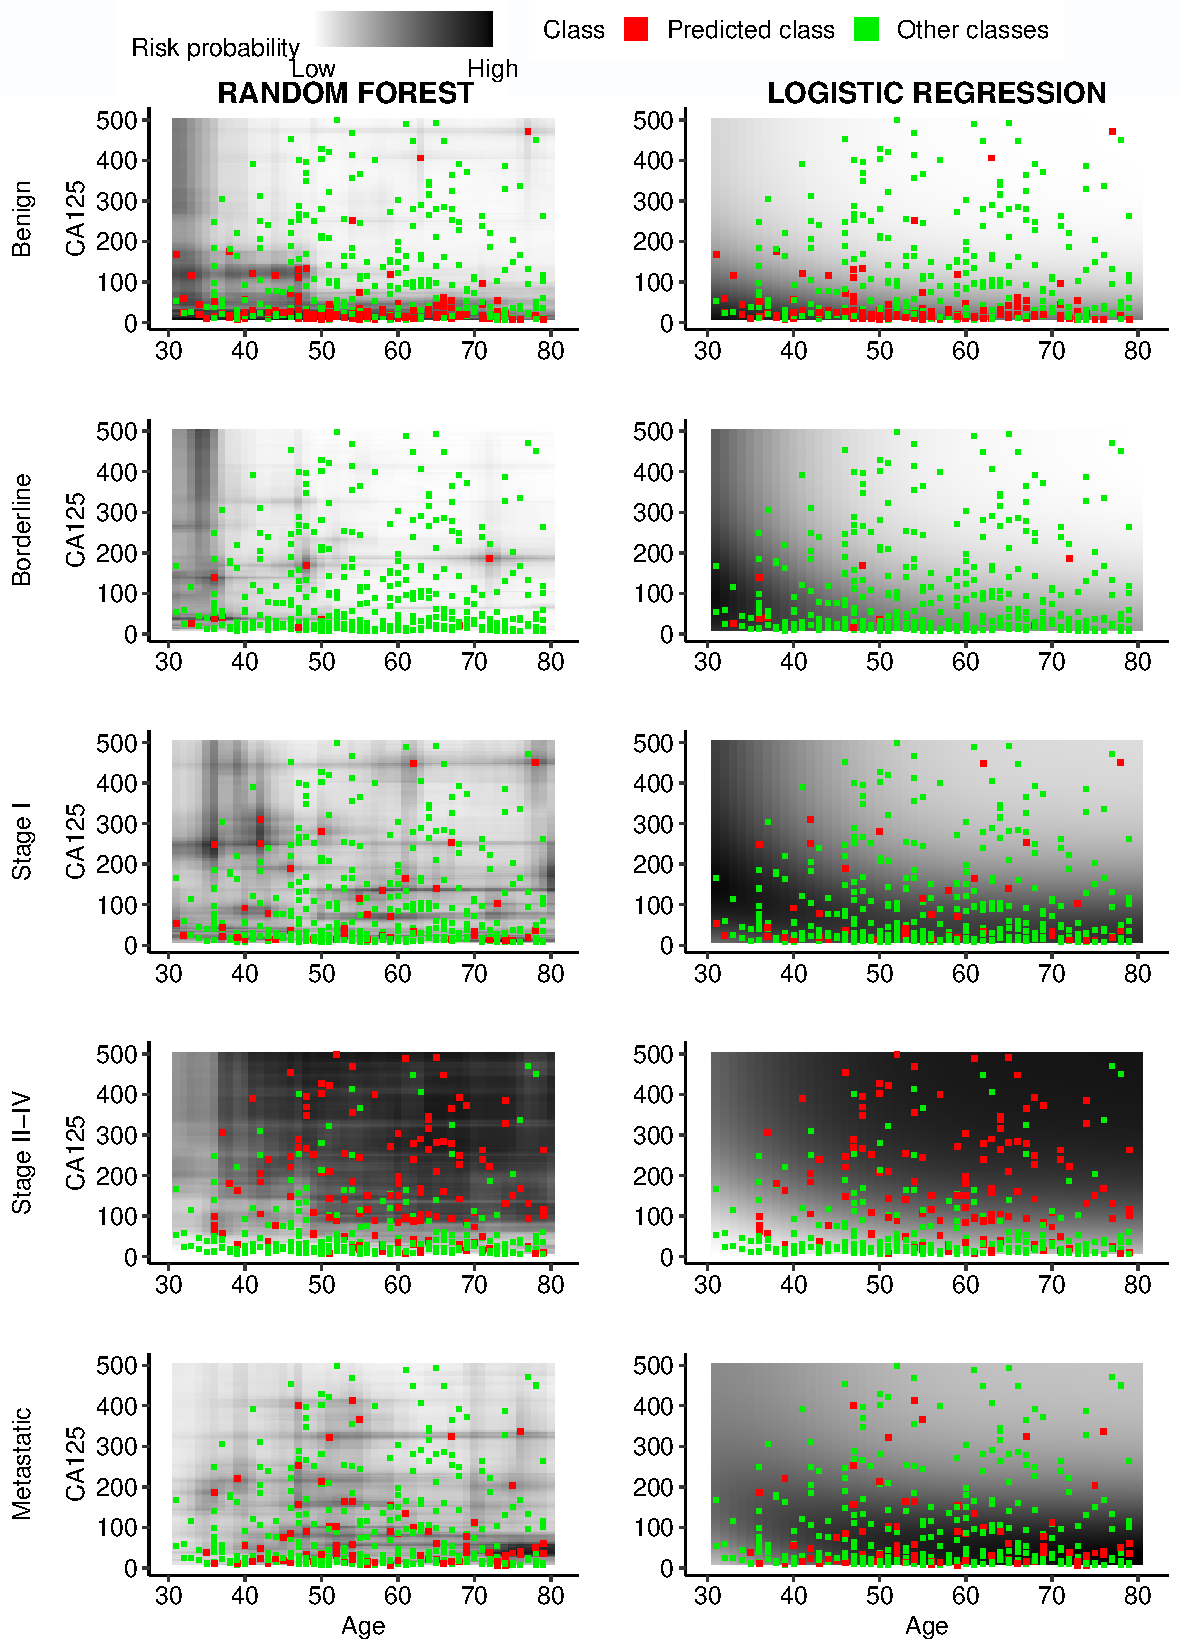
\includegraphics[width=1\textwidth]{figures/RFOverfitting/F1.pdf}
\caption[Heatmap of random forest and logistic regression predictions with training cases]{Random Forest and logistic regression probability estimation in data space for 4 subtypes of ovarian malignancy diagnosis with cases in training set superimposed. CA125 bounded to 500.}
\label{fig:3:1}
\end{figure}

\begin{figure}
\centering
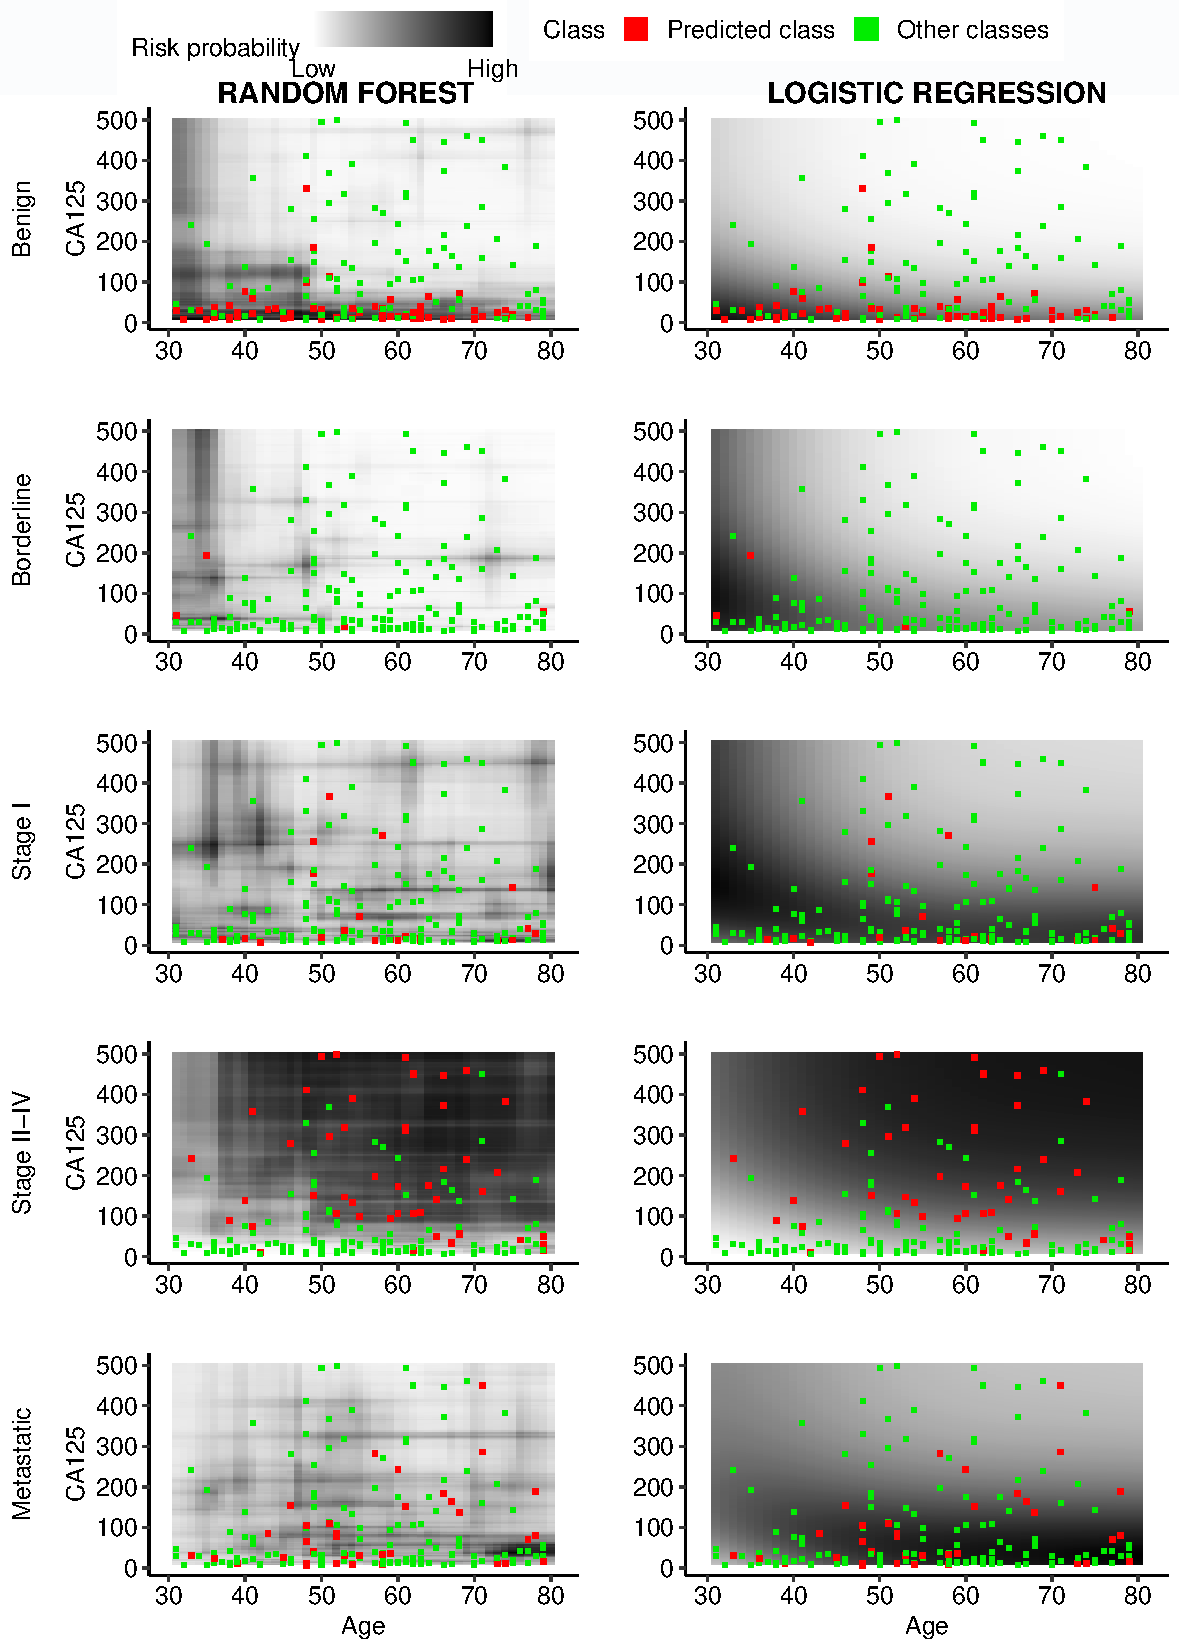
\includegraphics[width=1\textwidth]{figures/RFOverfitting/F2.pdf}
\caption[Heatmap of random forest and logistic regression predictions with test cases]{Random forest and logistic regression probability estimation in data space for 4 subtypes of ovarian malignancy diagnosis with cases in test set superimposed. CA125 bounded to 500.}
\label{fig:3:2}
\end{figure}

\begin{figure}
\centering
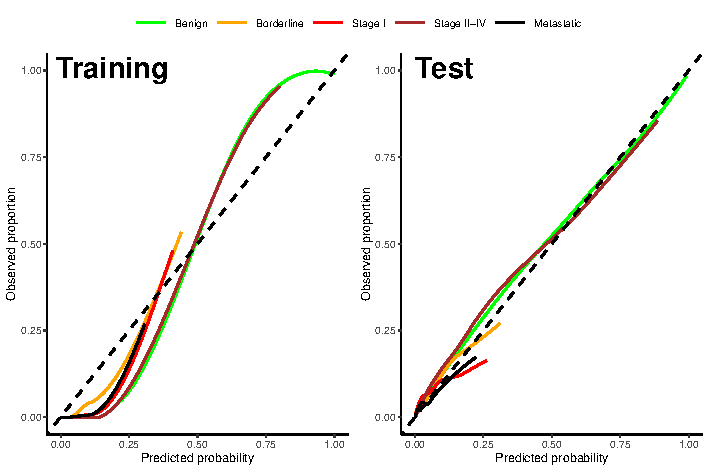
\includegraphics[width=1\textwidth]{figures/RFOverfitting/F3.pdf}
\caption[Calibration plots for random forest model]{Calibration plots for random forest model in ovarian cancer data. Observed proportion is estimated with a LOESS model. The plots only show observed proportions for predicted probabilities between quantiles 5th and 95th.}
\label{fig:3:3}
\end{figure}

\subsection{CRASH3: traumatic brain injury prognosis}
\gls{CRASH}-3 data was collected between 2012 and 2019 for a multicenter, randomized,
placebo-controlled trial to measure the effects of tranexamic acid on death,
disability, vascular occlusive events, and other morbidities in 12,660 patients
with acute traumatic brain injury (\gls{TBI})
 \cite{collaboratorsEffectsTranexamicAcid2019}. We used age (years) and systolic
blood pressure (mmHg) as continuous variables and sex, Glasgow Coma Scale (\gls{GCS})
eye-opening (4 levels), and pupillary reaction (4 levels) as categorical
variables. We performed a complete case analysis (\gls{CCA}) removing patients for
which one or more values were missing obtaining a complete dataset of 12,548
patients. \gls{CCA} was used for simplicity and because the phenomenon under study
should not be affected importantly by this. The outcome was measured 28 days
after randomization: alive ($n = 10{,}022$, 80\%), death due to head injury ($n
= 2309$, 18\%), or death of other cause ($n = 217$, 2\%) (detailed information
in Table S3). The training set included 8783 patients (70\%), and the test set
was 3765 (30\%).

For \gls{RF}, the \gls{PDI} was 0.96 in train data and 0.54 in test data. For \gls{MLR}, the \gls{PDI}
was 0.61 and 0.60, respectively. The heatmaps drew a similar picture compared
with the previous case study: \gls{RF} had clear probability peaks whilst \gls{MLR} had
smoothly changing probabilities (Figures S5--S8). The calibration plots for \gls{RF}
were also similar: poor calibration in training data but decent in the test data
for the 2 most common outcomes (Figure S9).

\subsection{IST: type of stroke diagnosis}
The International Stroke Trial (\gls{IST}) database was designed with the aim of
establishing whether early administration of aspirin, heparin, or both or
neither influenced the clinical course of acute ischaemic stroke
 \cite{sandercockInternationalStrokeTrial2011}. Data for the 19,435 patients with
suspected acute ischaemic stroke were recruited between 1992 and 1996. We use
age (years) and systolic blood pressure (mmHg) as continuous variables, and
conscious state (fully alert vs drowsy), deficit of face (yes vs no), deficit of
arm/hand (yes vs no), deficit of leg/foot (yes vs no), dysphasia (yes vs no),
and hemianopia (yes vs no) as categorical variables. We again performed a \gls{CCA}
retaining 15,141 patients. The outcome is the type of stroke: ischaemic ($n =
13{,}622$, 90\%), indeterminate ($n = 736$, 5\%), hemorrhagic ($n = 439$, 3\%),
or no stroke ($n = 344$, 2\%) (detailed information in Table S4). The training
set included 10,598 patients (70\%), and the test set 4543 (30\%).

The \gls{RF} model had a training \gls{PDI} of 0.89 and a test \gls{PDI} of 0.35. For \gls{MLR}, the
training set \gls{PDI} was 0.39, the test set \gls{PDI} was 0.41. In this dataspace, the
phenomenon is notorious, with very local peaks around train cases
(Figures S10-S13). The calibration plots for training and test data showed poor
calibration (Figure S14).

\section{Simulation study}
\label{sec:3.4}

\subsection{Aim}
We conducted a simulation study to assess which key factors of the modeling
setup (dataset and minimum node size) contribute to the phenomenon of having an
exaggerated \gls{AUC} in the training data without strong signs of overfitting in test
data. We report the simulation study using the \gls{ADEMP} (aims, data-generating
mechanisms, estimands, methods, and performance measures) structure
 \cite{morrisUsingSimulationStudies2019}. The code for the simulation study can
be found in the \gls{OSF} repository (\url{https://osf.io/y5tqv/}).

\subsection{Data-generating mechanism (DGM)}
For the simulation study, we generated data by assuming that the true model was
in the form of an \gls{MLR} with an outcome event fraction of 0.2 (see Additional
file 1: Appendix 1: Simulation Algorithm for details).

The 48 \glspl{DGM} differed according to the following parameters:
\begin{enumerate}[label=(\roman*)]
\item \textit{Predictor distribution}: predictors were either all continuous
with multivariate normal distribution or all binary with 50\% prevalence.
\item \textit{Number of predictors}: there were either 4 true predictors (0
noise predictors), 16 true predictors (0 noise predictors), or 16 predictors of
which 12 noise predictors. Noise predictors had a true regression coefficient
of~0.
\item \textit{Correlation between predictors}: Pearson correlations between all
predictors were either 0 or 0.4.
\item \textit{True AUC}: this was either 0.75 or 0.90.
\item \textit{Balance of regression coefficients}: the true model coefficients
that were not 0 were either all the same (balanced) or not (imbalanced). When
imbalanced, one-fourth of the predictors have a coefficient that is 4 times
larger than the others.
\end{enumerate}

The true model coefficients for generating the data were obtained by trial error
and are available in Table S5.

\subsection{Estimands}
For both training and test data, we estimate model discrimination, whether risk
estimates have too high (overconfidence) or too low (underconfidence) spread and
the prediction error. Underconfidence reflects the situation in Figure \ref{fig:3:3}
(Train): high probabilities are underestimated, and low probabilities are
overestimated. Overconfidence is the opposite: high probabilities are
overestimated, and low probabilities are underestimated. For test data, we also
calculate discrimination loss vs the true model and the relative contribution of
bias and variance to the prediction error. As the training and test samples are
based on the same \gls{DGM}, the test results reflect internal rather than external
validation.

\subsection{Methods}
We fitted models on training datasets of size 200 (small) or 4000 (large), and
for \gls{RF} models we used values for \textit{min.node.size} of 2 or 20 and ranger
package for training. As a result, there were $2 \times 2 \times 3 \times 2
\times 2 \times 2 \times 2 = 192$ scenarios. For each scenario, 1000 simulation
runs were performed (i.e., 1000 different training datasets). For \gls{RF},
\textit{ntree} was fixed at 500, and \textit{mtry} at the square root of the
number of predictors (default value). Models were validated on a single large
test dataset per \gls{DGM} ($N = 100{,}000$) to avoid sampling variability.

\subsection{Performance}
For discrimination we calculated the \gls{AUC} and for confidence of risk estimates
the calibration slope (slope $< 1$ means overconfidence, slope $> 1$
underconfidence). The calibration slope is calculated as the slope of a logistic
regression (\gls{LR}) model fitting the outcome to the logit of the estimated
probabilities as the only predictor. Calibration intercept is calculated fitting
the same model for a slope of 1 by setting the predicted probabilities as an
offset term. Discrimination loss was calculated as the difference between true
\gls{AUC} and median test \gls{AUC}. Finally, the mean squared error (\gls{MSE}) of the predicted
probabilities was calculated according to \cite{friedmanBiasVariance02004} as
the sum of squared bias and variance (see Additional file 1: Appendix 2:
Simulation metrics for details).

\section{Results}

The aggregated simulation results using median and interquartile range for
discrimination and calibration and mean and standard deviation for mean squared
error are available in Additional file 1 (Table S6). The complete simulation
including the code and 1000 simulations for each of the 192 scenarios is
available in the \gls{OSF} repository \cite{barrenadaUnderstandingOverfittingRandom2023}.

\subsection{Discrimination}
In the simulation study, the median training \glspl{AUC} were close to 1 in most of
the cases. The median training \gls{AUC} was between 0.97 and 1 unless there were 4
binary predictors, or 16 binary predictors combined with a minimum node size of
20 (Figure \ref{fig:3:4}). Higher \textit{min.node.size} resulted in less extreme training
\glspl{AUC}.

\begin{figure}
\centering
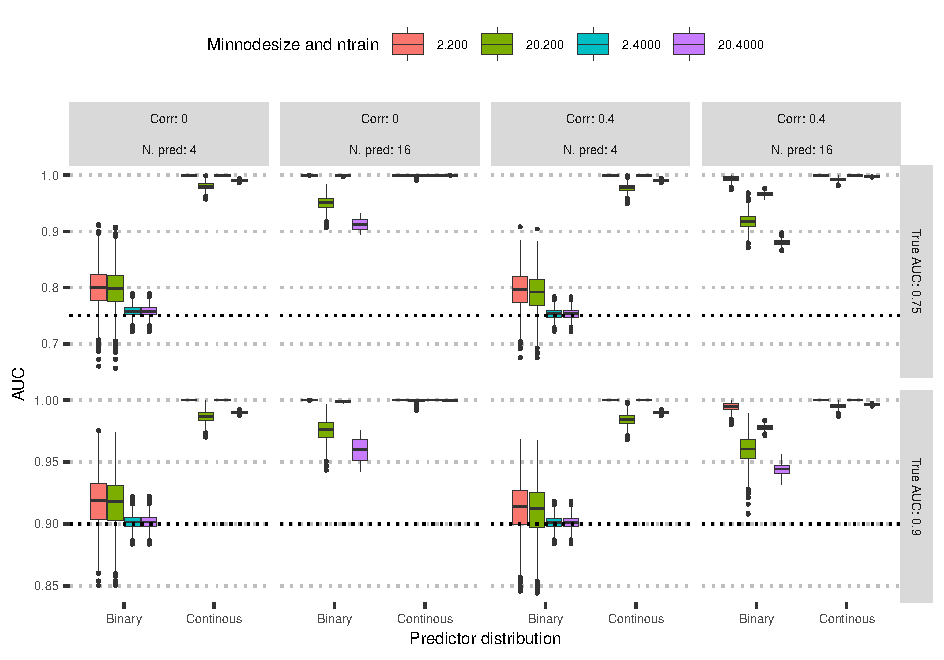
\includegraphics[width=1\textwidth]{figures/RFOverfitting/F4.pdf}
\caption[Simulation training AUC]{Training AUC by simulation factors and modeling hyperparameters in scenarios without noise. Scenarios are aggregated by strength because this simulation factor had minimal effect.}
\label{fig:3:4}
\end{figure}

In general, median test \glspl{AUC} were higher when there was a large vs small
training dataset, high vs low \textit{min.node.size}, high vs low correlation
between predictors, binary versus continuous predictors, and 4 versus 16
predictors (except with correlated continuous predictors) (Figure \ref{fig:3:5}). All other
simulation factors being equal, the scenarios with 4 true and 12 noise
predictors had results for the \gls{AUC} that was identical to scenarios with 16
predictors (Figures \ref{fig:3:4} and \ref{fig:3:5} and S15-16).

\begin{figure}
\centering
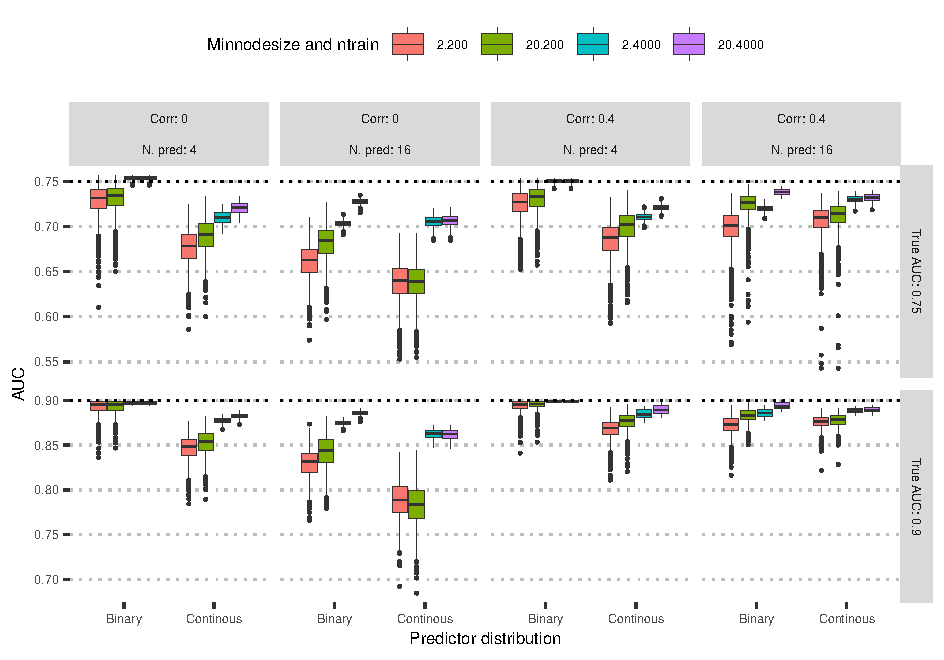
\includegraphics[width=1\textwidth]{figures/RFOverfitting/F5.pdf}
\caption[Simulation test AUC]{Test AUC by simulation factors and modeling hyperparameters in scenarios without noise. Scenarios are aggregated by strength.}
\label{fig:3:5}
\end{figure}

The Spearman correlation between median training \gls{AUC} and discrimination loss was
0.72 for scenarios with a true \gls{AUC} of 0.9, and 0.69 for scenarios with a true
\gls{AUC} of 0.75 (Figure S17). The median discrimination loss was 0.025 (range 0.00
to 0.13). In the 114 scenarios where the median training \gls{AUC} was $\geq 0.99$,
the median discrimination loss was 0.036 (range 0.003 to 0.13). In the other
scenarios, the median discrimination loss was 0.013 (0.00 to 0.069).

\subsection{Calibration}
Median training calibration slopes ranged between 1.10 and 19.4 (Figure \ref{fig:3:6} and
Figure S18): the probability estimates were always underconfident where high
probabilities were underestimated and low probabilities overestimated. This is
the consequence of perfect separation between events and non-events in training
data (i.e., \gls{AUC} $= 1$) which means that any estimation above 0 or below 1 is
underconfident (Figure S19). The median slope was lowest in scenarios with few
binary predictors or higher \textit{min.node.size}. Median test calibration
slopes ranged between 0.45 and 2.34. Across all scenarios, the Spearman
correlation between the median training slope and median test slope was $-0.11$
(Figure S17). Median test slopes were mainly higher when the true \gls{AUC} or
\textit{min.node.size} was higher. In addition, median test slopes tended to be
higher with binary predictors, uncorrelated predictors, and higher sample sizes
(Figure \ref{fig:3:7} and Figure S18). Calibration slopes were similar in scenarios with 16
true predictors, 4 true predictors, and 12 noise predictors (Figures \ref{fig:3:6} and \ref{fig:3:7}
and Figures S20-21). In the 78 scenarios without perfect training (\gls{AUC} $<
0.99$) the median test calibration slope was between 0.59 and 2.34 with a
median of 1.10. In the 114 scenarios with almost perfect training \gls{AUC} ($\geq
0.99$), the median calibration slope was 0.92.

\begin{figure}
\centering
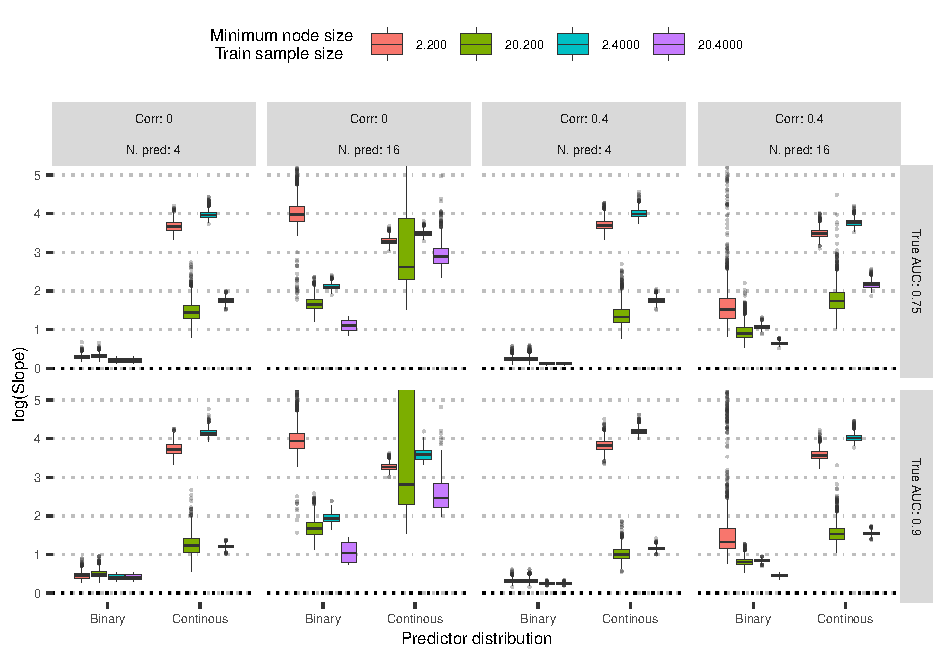
\includegraphics[width=1\textwidth]{figures/RFOverfitting/F6.pdf}
\caption[Simulation training calibration log slope]{Training set calibration log slope by simulation factors and modeling hyperparameters in scenarios without noise. Scenarios are aggregated by strength. The ideal value for the log slope is 0.}
\label{fig:3:6}
\end{figure}

\begin{figure}
\centering
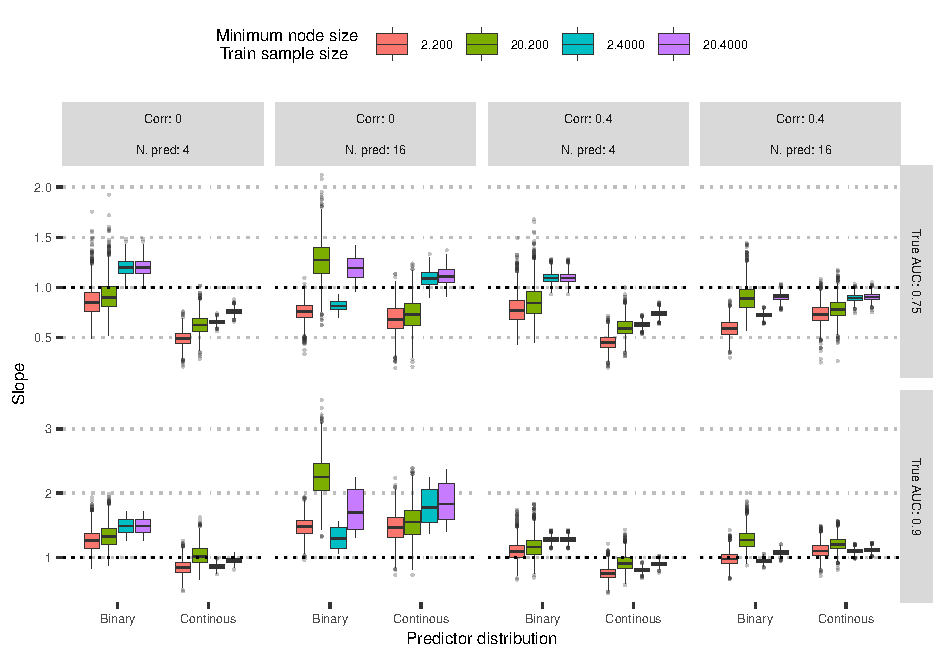
\includegraphics[width=1\textwidth]{figures/RFOverfitting/F7.pdf}
\caption[Simulation test calibration slope]{Test set calibration slope by simulation factors and modeling hyperparameters in scenarios without noise. Scenarios are aggregated by strength. The ideal value for the slope is 1.}
\label{fig:3:7}
\end{figure}

\subsection{Mean squared error (MSE)}
Median \gls{MSE} across scenarios was 0.008 (range 0.000--0.045) with a median
squared bias of 0.002 (range 0.000--0.038) and median variance of 0.005 (range
0.000--0.017). For the 114 scenarios with median training \gls{AUC} $\geq 0.99$, we
observed a median test \gls{MSE} of 0.010 with a median squared bias of 0.004 (range
0.0004--0.0384) and a median variance of 0.006 (range 0.001--0.017). For the
rest of the scenarios, the median test \gls{MSE} was 0.006. Across all scenarios, the
Spearman correlation of mean test squared bias and mean test variance with
median training \gls{AUC} were 0.47 and 0.43, respectively. The correlation with the
discrimination loss was 0.51 for the squared bias and 0.70 for the variance.
Lower sample size in training was associated with higher median test variance,
and with higher median test squared bias in scenarios with continuous predictors.
Lower \textit{min.node.size} (i.e., deeper trees) was associated with a lower
variance but higher bias in test data when the training sample size was small.
More predictors were associated with higher bias, whereas the correlation
between predictors and higher true \gls{AUC} was associated with lower bias
(Figure \ref{fig:3:8}). The models with noise predictors had lower variance and higher bias
compared to scenarios with 4 true and no noise predictors (Figure S22).

\begin{figure}
\centering
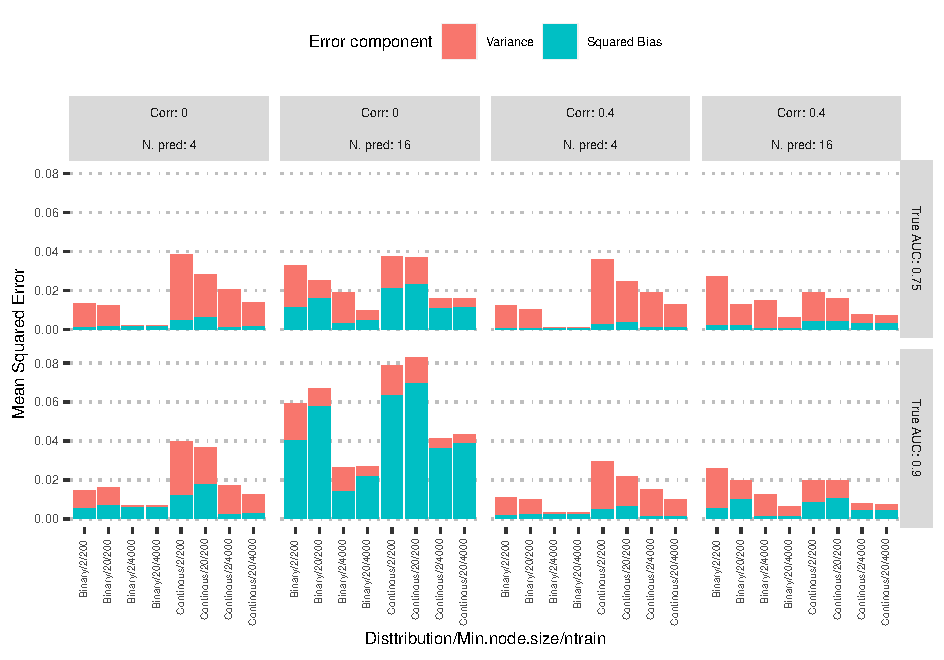
\includegraphics[width=1\textwidth]{figures/RFOverfitting/F8.pdf}
\caption[Simulation mean squared error]{Mean squared error across scenarios without noise aggregated by strength.}
\label{fig:3:8}
\end{figure}

\section{Overall discussion}
\label{sec:3.5}

We tried to better understand and visualize the behavior of random forests for
probability estimation. We make three key observations from this work. First, \gls{RF}
models learn local probability peaks around training set events, in particular
when the trees are very deep (i.e., low \textit{min.node.size}) and when there
are continuous predictors. Where a group of events is located close to one
another in ``data space'', the probability peaks are combined into a region of
increased probability. Where events are isolated in data space, the probability
peaks are very local. Learning through peaks leads to very optimistic (often
near perfect) discrimination in training data, but also to reduced
discrimination in new data compared to models that rely on less deep trees (cf.\
simulation settings where \gls{RF} models with \textit{min.node.size} 2 vs 20 were
fitted on a set of continuous predictors). Probably, the reduction in
discrimination on new data is modest because the local peaks for isolated events
are often harmless for new data: it is unlikely to see an event in the exact
same location. Second, \gls{RF} also suffers from ``classical overfitting'' in which
models with higher discrimination on training data tend to have lower
discrimination on new data than models with less optimistic discrimination (cf.\
simulation settings where \gls{RF} models are learned on 4 binary predictors using 200
vs 4000 training cases). Third, in training and test data, calibration
performance for \gls{RF} models is different from what we commonly observe for \gls{LR}
models. Whereas \gls{LR} based on maximum likelihood leads by definition to
calibration slopes of 1 on training data, calibration slopes for \gls{RF} models were
always above 1 on training data. Also, as opposed to \gls{LR}, calibration slopes for
\gls{RF} models do not converge to 1 on new data. This different behavior is probably
caused by the pragmatic way in which probabilities are obtained for \gls{RF} models,
whilst \gls{LR} estimates probabilities in a principled way through maximum
likelihood.

The simulation results regarding discrimination and calibration go against
fitting very deep trees when using \gls{RF} for probability estimation. This is in
line with recent work that illustrated that \gls{RF} using deeply grown trees results
in risk estimates that are particularly unstable
 \cite{rileyStabilityClinicalPrediction2023}. The heatmaps for our case studies
illustrate how \gls{RF} models with deeply grown trees lead to probabilities that
change non-smoothly with changes in the values of predictors. It has been
suggested to set \textit{min.node.size} to 5\% or 10\% of the sample size
 \cite{malleyProbabilityMachinesConsistent2012,kruppaConsumerCreditRisk2013}.
Alternatively, \textit{min.node.size} can be tuned. Although this was not the
focus of our study, it seems natural to tune with logloss (also known as the
negative loglikelihood or cross-entropy) or Brier score as the loss function
since they capture calibration
 \cite{probstHyperparametersTuningStrategies2019}. In their work, Ledger and
colleagues tuned \textit{min.node.size} by optimizing logloss based on tenfold
cross-validation for 30 random values for mtry and \textit{min.node.size} using
the trainControl and train functions from the caret R package
 \cite{ledgerMulticlassRiskModels2023}. This resulted in $\textit{mtry} = 3$ and
$\textit{min.node.size} = 15$, with competitive results in test data. Applying
the tuneRanger R package with 200 iterations for our case studies based on
logloss yielded an optimal \textit{min.node.size} of 8 (0.1\% of training set
size) for ovarian cancer data, 261 (2.1\%) for \gls{CRASH}3 data and 591 (3.9\%) for
\gls{IST} data \cite{probstHyperparametersTuningStrategies2019}. These values are
higher than the default values in many statistical software programs.

Three comments regarding the interpretation of discrimination and calibration
results for \gls{RF} models are worth making. First, it is well known that apparent
performance, i.e., performance assessment on the exact same dataset that was
used to train the model, is overly optimistic
 \cite{altmanWhatWeMean2000,moonsPROBASTToolAssess2019}. Our work indicates that
this is a fortiori case for \gls{RF}. Unfortunately, some studies present their \gls{RF}
models with ``excellent'' performance because they only present discrimination
for the training data
 \cite{daiUsingRandomForest2018,chenPredictionMalignantMiddle2015,yuanDevelopmentHeartFailure2019}.
Instead, proper internal and external validation results should be reported.
Second, from a regression modeling perspective, a calibration slope that is
clearly below 1 on internal validation is a symptom of overfitting. This cannot
be applied in the same way for \gls{RF} models. Models based on larger training
samples had higher calibration slopes in our simulation study, but a calibration
slope of 1 does not appear to have a special meaning. Models with a calibration
slope above 1 on test data when trained on 200 training samples, had an even
higher slope when trained on 4000 samples. The interpretation of risk estimates
based on \gls{RF} requires caution, probably because probabilities are generated in a
very ad hoc way. Of course, the calibration slope still quantifies in a
descriptive manner whether the risk estimates are on average too confident
(slope $< 1$), not confident enough (slope $> 1$), or fine (slope $= 1$).
Third, despite that \gls{RF} models had high discrimination results in the training
data (suggestive of overfitting), the calibration slope in the training data was
always above 1 (risk estimates show too little spread, suggestive of
underfitting). This appears to be a consequence of the bootstrapping procedure
in combination with the low \textit{min.node.size}. Due to the bootstrapping, a
training set case was part of approximately 63\% of bootstrap samples and
therefore was used for 63\% of the trees in the forest. When averaging the
proportion of events in the appropriate leaf nodes over all \textit{ntree} trees
to get a probability estimate for a given training set case, 63\% of these
proportions are near perfect: close to 1 if the training case is an event,
close to 0 if the training cases is a non-event. The remaining 37\% are more
variable and often far less good. The 63\% near-perfect proportions cause
discrimination to be very high because most events will end up with an estimated
probability of an event that is higher than that for most non-events. The
remaining 37\% of the proportions pull the probability estimates away from 0 (if
the case is a non-event) or 1 (if the case is an event), leading to calibration
slopes $> 1$.

Although the aim of our paper was largely educational, it links to previous more
fundamental work and fills a gap in the literature by explicitly studying
factors that contribute to better discrimination and calibration of new data.
Wyner and colleagues (2017) argued that \gls{RF} has excellent performance because it
is an ``interpolating classifier'', i.e., it is fitted with little to no error
to the train data \cite{wynerExplainingSuccessAdaBoost2017a}. They argue that
the interpolation should not be confused with overfitting. Even if the
individual trees are overfitting, each training set case is not used in about
37\% of the individual trees, such that averaging over trees partially solves
overfitting. Belkin and colleagues have linked this to a double descent curve
for highly flexible algorithms: when the complexity of the model increases, test
set performance first improves, then deteriorates, and finally improves again
once the ``interpolation threshold'' (where perfect training performance is
achieved) is exceeded \cite{belkinFitFearRemarkable2021}. Recently, however,
Buschjäger and Morik opposed the existence of double descent in \gls{RF}
 \cite{buschjagerThereNoDoubleDescent2021}. Mentch and Zhou linked the success of
\gls{RF} to the signal-to-noise ratio (\gls{SNR}) of the data. In their work, they present
that the randomness of \gls{RF} is beneficial in situations with low \gls{SNR} whereas
bagging is preferred if \gls{SNR} is high
 \cite{mentchRandomizationRegularizationDegrees2020}. They explain the success of
\gls{RF} by the low \gls{SNR} of many real-world datasets. This view contradicts the view
that flexible algorithms work best when the \gls{SNR} is high
 \cite{vancalsterMachineLearningMedicine2019}. Finally, the issue of calibration
of estimated probabilities in the context of \gls{RF} models received little attention
in the literature, although it is key for optimal clinical decision making
 \cite{vancalsterCalibrationRiskPrediction2015}. It has been suggested that using
fully grown trees in \gls{RF} leads to suboptimal risk estimates
 \cite{malleyProbabilityMachinesConsistent2012,kruppaConsumerCreditRisk2013}.
However, this is rarely mentioned and hence it is common to see that low minimum
node sizes are recommended because the problem is treated as a classification
problem instead of a probability estimation problem (e.g., see default for
randomForest package or scikit-learn). We think that the current study sheds
further light on probability estimation in \gls{RF}. Of course, a generic alternative
that works for any miscalibrated model is to recalibrate the probabilities of
the \gls{RF} afterward using new data
 \cite{ojedaCalibratingMachineLearning2023}.

We identified the following limitations of our study. Firstly, a simulation
study is always limited by the included scenarios. It would be of interest to
include more simulation factors and values per simulation factor (e.g., for
\textit{min.node.size}) in the simulation study or to include scenarios where \gls{RF}
hyperparameters are tuned rather than fixed. Tuning could improve the
calibration of the models
 \cite{probstHyperparametersTuningStrategies2019,kruppaProbabilityEstimationMachine2014a}.
However, the simulation study already had 192 scenarios, and adding more factors
or values would increase the computational cost exponentially and would
overcomplicate the interpretation of the results. Topics that could be
investigated in further simulation studies include varying other hyperparameters
than \textit{min.node.size} (e.g., \textit{mtry}, sampling fraction, splitting
rule) and investigating more values for sample size, number of predictors, the
proportion of noise predictors, and min.node.size. Secondly, we were using
logistic \glspl{DGM} without nonlinear or nonadditive associations with the outcome. We
assumed that the impact of this would be limited, because the focus was not on
the comparison of \gls{RF} with \gls{LR}, and any nonlinearity or nonadditivity (including
the absence of it) has to be learned by the algorithm. Thirdly, the traditional
\gls{RF} algorithm selects variables at each split in a way that favors continuous
over binary variables \cite{stroblBiasRandomForest2007}. Continuous variables
can split in many ways, such that there is often a split that, perhaps by
chance, has a better Gini impurity reduction than the Gini impurity reduction
for a binary variable. The splits for continuous variables may often overfit,
thereby increasing training discrimination but decreasing test discrimination.
It is well documented that this affects variable importance measures
 \cite{stroblBiasRandomForest2007}, but it may also be relevant for model
performance. The problem can be addressed by using an adapted \gls{RF} algorithm such
as cforest from the partykit package
 \cite{hothornUnbiasedRecursivePartitioning2006}. These adapted algorithms grow
conditional inference trees (\gls{CIT}) instead of classification trees. For the case
studies, we observed that tuning and using the adapted \gls{RF} yields a less
optimistic training \gls{AUC} and similar or slightly better test performance (see \gls{OSF}
Repository \cite{barrenadaUnderstandingOverfittingRandom2023}. However, our aim was to understand
how the characteristics of the data and the modeling process affected the
models, hence we did not systematically explore the effects of tuning or
alternative algorithms.

We conclude that \gls{RF} tends to exhibit local overfitting by learning probability
peaks, in particular when the \gls{RF} model is based on deeply grown trees. This
local overfitting can lead to highly optimistic (near perfect) discrimination on
the training data but to reduced discrimination on new data compared to \gls{RF}
models based on less deeply grown trees. In line with the work of Kruppa and
colleagues \cite{kruppaProbabilityEstimationMachine2014a}, our results go
against the recommendation to use fully grown trees when using \gls{RF} for
probability estimation.

\section*{Availability of data and materials}
All data and code that support the findings of this study are openly available
in the \gls{OSF} repository
 \cite{barrenadaUnderstandingOverfittingRandom2023} except the ovarian cancer
dataset which is not publicly available.

\section*{Acknowledgements}
Partial findings from this paper were presented at the Young Statisticians
Meeting 2023 in Leicester (July) and in the Conference of the International
Society of Clinical Biostatistics (ISCB) 2023 in Milan (August).

\section*{Other information}
\subsection*{Funding}
This research was supported by the Research Foundation--Flanders (FWO) under
grant G097322N with BVC and DT as supervisors.

\subsection*{Conflicts of interest}
The authors declare that they have no competing interests.

\subsection*{Contributors}
Contributions were based on the CRediT taxonomy. Conceptualization: LB, BVC.
Funding acquisition: BVC, DT. Project administration: LB. Supervision: BVC.
Methodology: LB, PD, ALB, BVC. Resources: LB, DT, BVC. Investigation: LB, PD,
DT, ALB, BVC. Validation: LB, BVC. Data curation: LB. Software: LB, BVC.
Formal analysis: LB, BVC. Visualization: LB, BVC. Writing---original draft: LB,
BVC. Writing---review and editing: all authors. All authors have read, share
final responsibility for the decision to submit for publication, and agree to be
accountable for all aspects of the work.
